% Digital Logic Report Template
% Created: 2020-01-10, John Miller

%==========================================================
%=========== Document Setup  ==============================

% Formatting defined by class file
\documentclass[11pt]{article}

% ---- Document formatting ----
\usepackage[margin=1in]{geometry}	% Narrower margins
\usepackage{booktabs}				% Nice formatting of tables
\usepackage{graphicx}				% Ability to include graphics

%\setlength\parindent{0pt}	% Do not indent first line of paragraphs 
\usepackage[parfill]{parskip}		% Line space b/w paragraphs
%	parfill option prevents last line of pgrph from being fully justified

% Parskip package adds too much space around titles, fix with this
\RequirePackage{titlesec}
\titlespacing\section{0pt}{8pt plus 4pt minus 2pt}{3pt plus 2pt minus 2pt}
\titlespacing\subsection{0pt}{4pt plus 4pt minus 2pt}{-2pt plus 2pt minus 2pt}
\titlespacing\subsubsection{0pt}{2pt plus 4pt minus 2pt}{-6pt plus 2pt minus 2pt}

% ---- Hyperlinks ----
\usepackage[colorlinks=true,urlcolor=blue]{hyperref}	% For URL's. Automatically links internal references.

% ---- Code listings ----
\usepackage{listings} 					% Nice code layout and inclusion
\usepackage[usenames,dvipsnames]{xcolor}	% Colors (needs to be defined before using colors)

% Define custom colors for listings
\definecolor{listinggray}{gray}{0.98}		% Listings background color
\definecolor{rulegray}{gray}{0.7}			% Listings rule/frame color

% Style for Verilog
\lstdefinestyle{Verilog}{
	language=Verilog,					% Verilog
	backgroundcolor=\color{listinggray},	% light gray background
	rulecolor=\color{blue}, 			% blue frame lines
	frame=tb,							% lines above & below
	linewidth=\columnwidth, 			% set line width
	basicstyle=\small\ttfamily,	% basic font style that is used for the code	
	breaklines=true, 					% allow breaking across columns/pages
	tabsize=3,							% set tab size
	commentstyle=\color{gray},	% comments in italic 
	stringstyle=\upshape,				% strings are printed in normal font
	showspaces=false,					% don't underscore spaces
}

% How to use: \Verilog[listing_options]{file}
\newcommand{\Verilog}[2][]{%
	\lstinputlisting[style=Verilog,#1]{#2}
}




%======================================================
%=========== Body  ====================================
\begin{document}

\title{ELC 2137 Lab 9: ALU with Input Register }
\author{Mariah Montgomery}

\maketitle


\section*{Summary}

Type the summary of your experiment and results here.  


\section*{Q\&A}

\begin{table*}[ht]\centering
	\caption{\textit{Register} Expected Results Table}
	\label{ALU:tbl:register_ERT}\medskip
	\begin{tabular}{l|rrrrrrrrrrr}
		Time (ns): & 0-5 & 5-10 & 10-15 & 15-20 & 20-25 & 25-30 & 30-35 & 35-40 & 40-45 & 45-50 & 50-55 \\
		\midrule
		D (hex) & 0 & 0 	  & A & A & 3 	    & 3 	  & 0 	    & 0 & 0$\to$6 & 6 & 6 \\
		clk     & 0 & 1 	  & 0 & 1 & 0 	    & 1 	  & 0 	    & 1 & 0 	  & 1 & 0 \\
		en  	& 0 & 0 	  & 1 & 1 & 1$\to$0 & 0$\to$1 & 1$\to$0 & 0 & 0$\to$1 & 1 & 1 \\
		rst 	& 0 & 0$\to$1 & 0 & 0 & 0 		& 0 	  & 0		& 0 & 0		  & 0 & 0 \\
		\midrule
		Q (hex) & X & X$\to$0 & 0 & A & A & A & A & A & A & 6 & 6 \\
		\bottomrule
	\end{tabular}
\end{table*}

\begin{table*}[ht]\centering
	\caption{\textit{ALU} Expected Results Table}
	\label{ALU:tbl:alu_ERT}\medskip
	\begin{tabular}{l|rrrrrr}
		Time (ns): & 0-10 & 10-20 & 20-30 & 30-40 & 40-50 & 50-60 \\
		\midrule
		in0 & 0111 & 0111 & 0111 & 0111 & 0111 & 0111 \\
		in1 & 0001 & 0001 & 0001 & 0001  & 0001 & 0001 \\
		op	& 0 & 1  & 2 & 3 & 4 & 5  \\
		\midrule
		out & 1000  & 0110 & 0001 & 0111  & 0110 & 0111 \\
		\bottomrule
	\end{tabular}
\end{table*}


\section*{Results}
\begin{enumerate}
	
\item Register Test Simulation

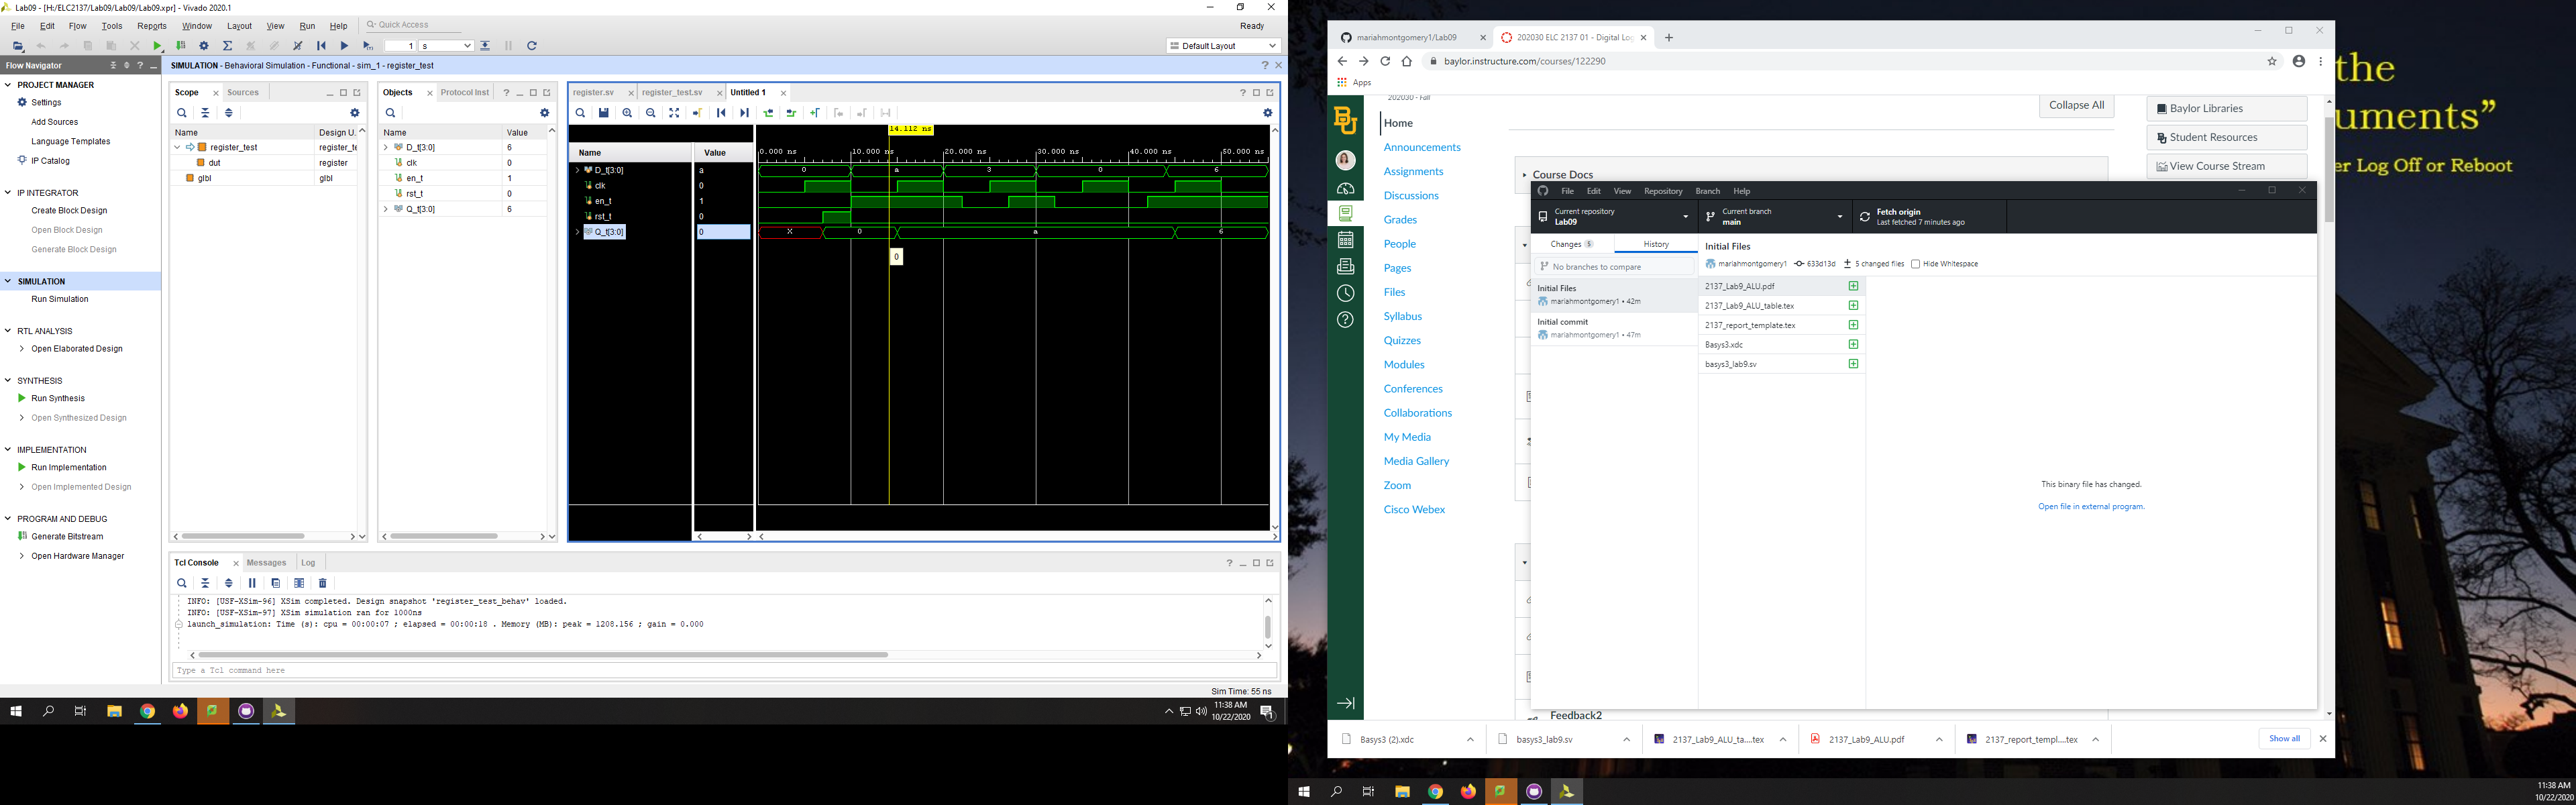
\includegraphics[width=0.8\textwidth, trim= 28.5cm 16cm 68cm 5.5cm, clip]{register_test.PNG}
\label{fig:Register Test Simulation}

\item ALU Test Simulation 

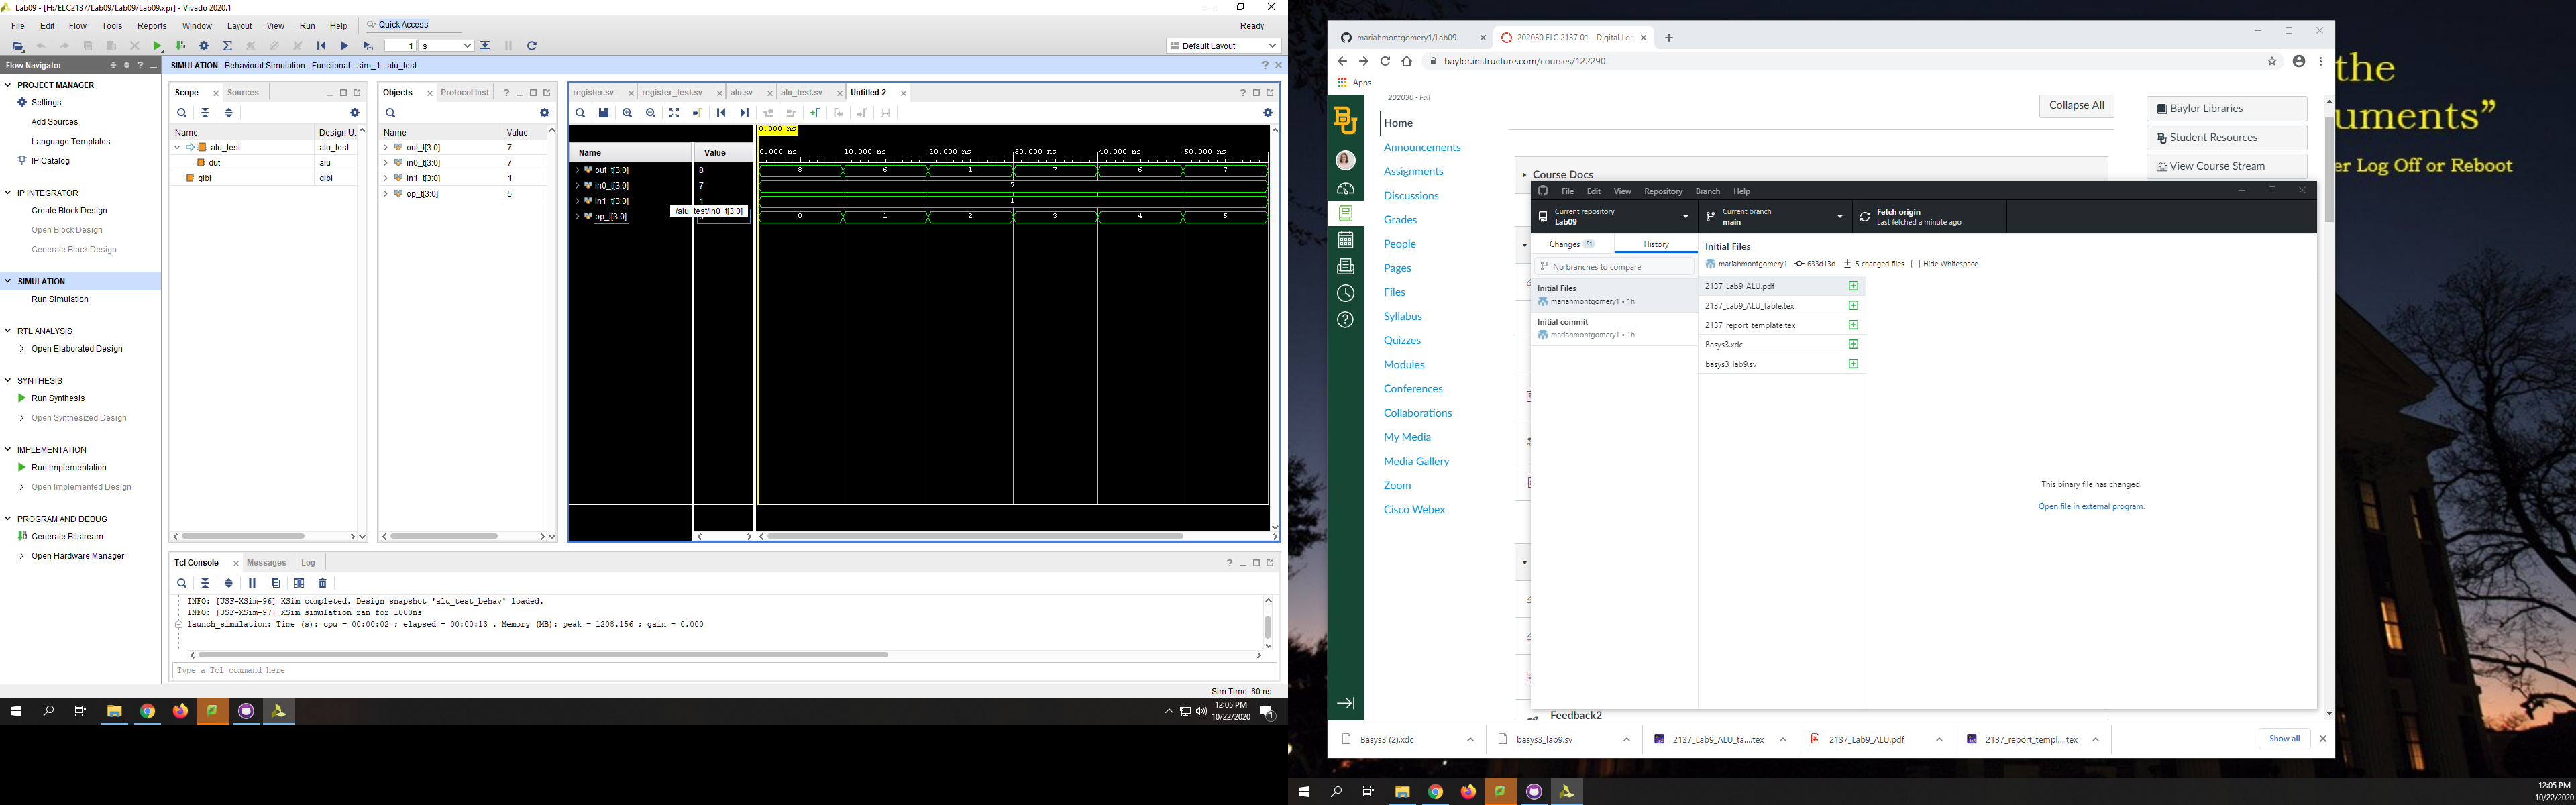
\includegraphics[width=0.8\textwidth, trim= 28.5cm 16cm 68cm 5.5cm, clip]{alu_test.PNG}
\label{fig:ALU Test Simulation}


\item Top-Level Simulation 

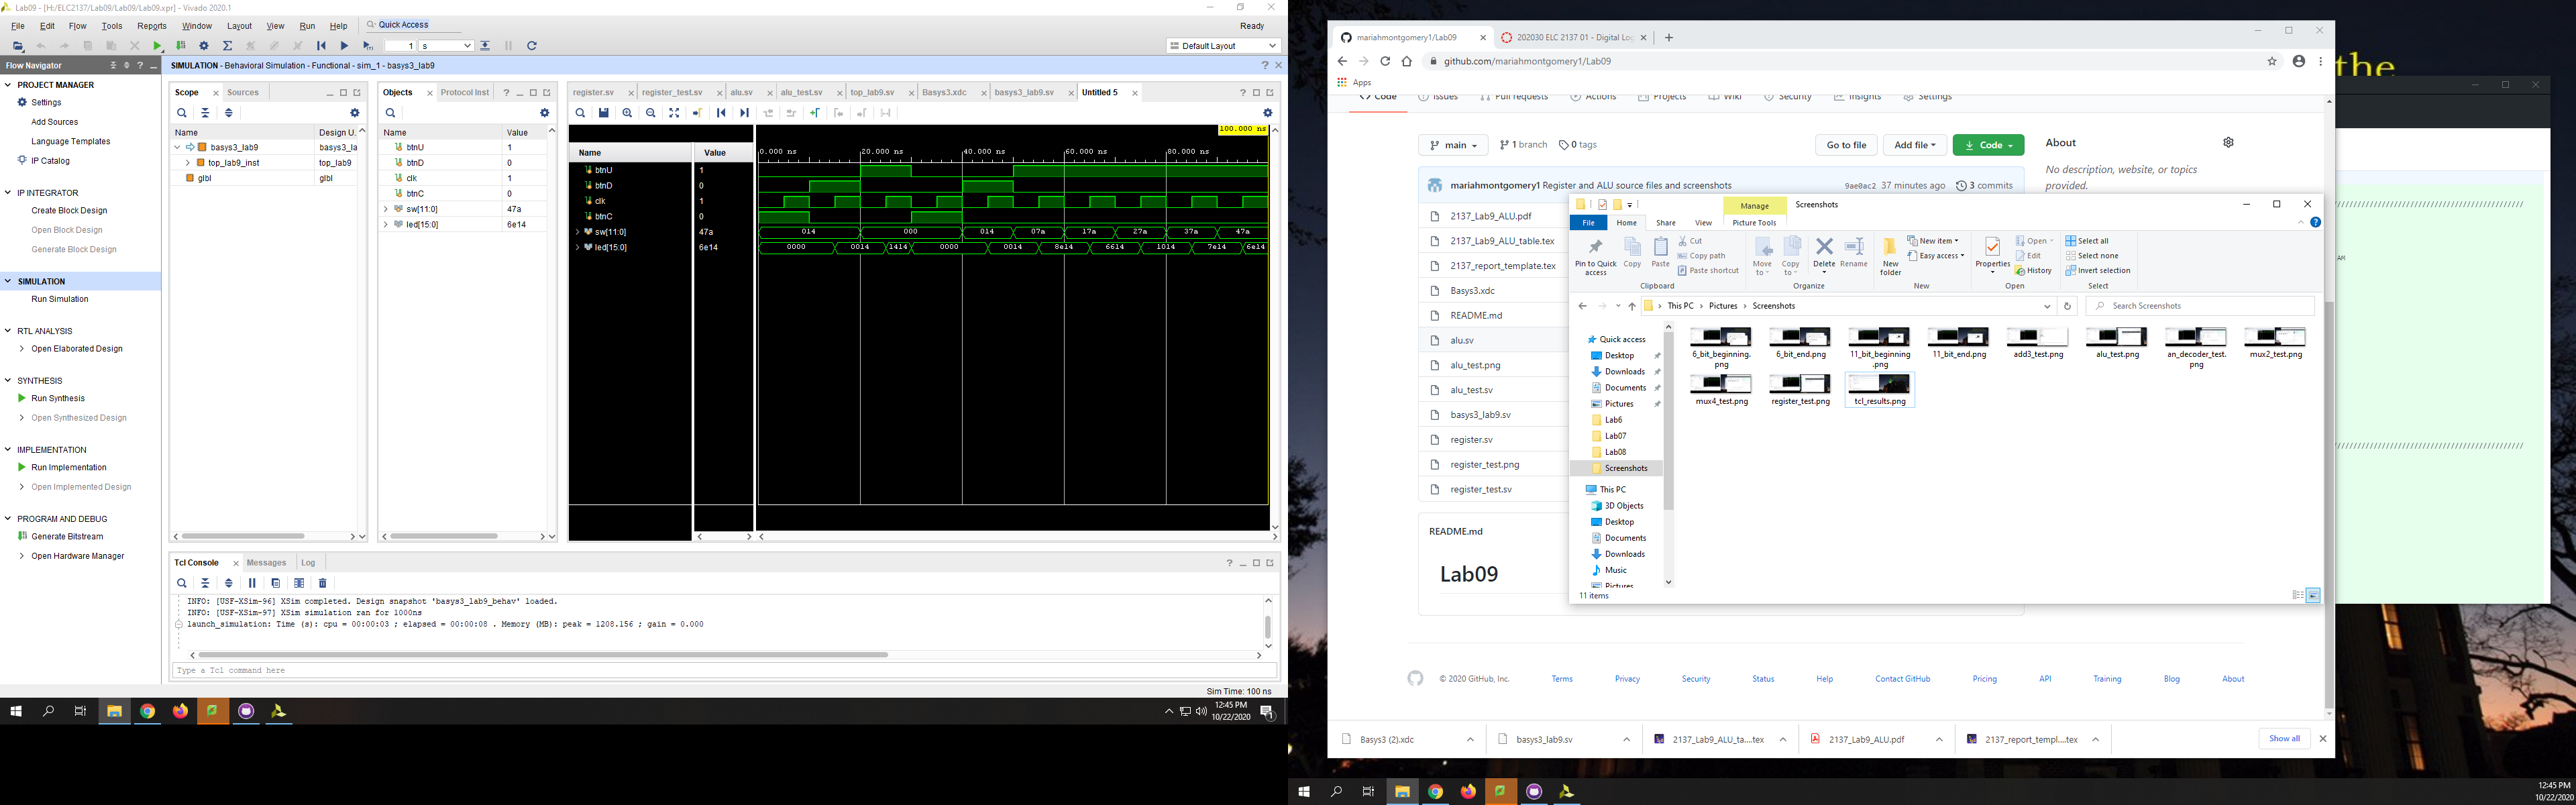
\includegraphics[width=0.8\textwidth, trim= 28.5cm 16cm 68cm 5.5cm, clip]{top_level_test.PNG}
\label{fig:Top-Level Simulation }

\end{enumerate}

\section*{Code}

\begin{lstlisting}[style=Verilog,caption=register ,label=register.sv]
module register #(parameter N=1)
	(
		input clk,
		input rst,
		input en,
		input [N-1:0] D,
		output reg [N-1:0] Q
	);

	always @(posedge clk, posedge rst)
	begin 
		if (rst == 1)
			Q <= 0;
		else if (en == 1)
			Q <= D;
	end 
endmodule
\end{lstlisting}

\begin{lstlisting}[style=Verilog,caption=Register Test,label=register_test.sv]
module register_test();

	reg [3:0] D_t;
	reg clk, en_t, rst_t;
	wire [3:0] Q_t;

	register #(.N(4)) dut(
		.D(D_t),
		.clk(clk),
		.en(en_t),
		.rst(rst_t),
		.Q(Q_t)
	);

	always begin 
		clk = ~clk; #5;
	end

	initial begin
		clk = 0; en_t = 0; rst_t = 0; D_t = 4'h0; #7; 
		rst_t = 1; #3;
		D_t = 4'hA; en_t = 1; rst_t = 0; #10;
		D_t = 4'h3; #2;
		en_t = 0; #5;
		en_t = 1; #3;
		D_t = 4'h0; #2;
		en_t = 0; #10;
		en_t = 1; #2;
		D_t = 4'h6; #11;
		$finish;
	end 
endmodule
\end{lstlisting}

\begin{lstlisting}[style=Verilog,caption=ALU ,label=alu.sv]
module alu #(parameter N=8) 
	(
		input [N-1:0] in0,
		input [N-1:0] in1,
		input [3:0] op,
		output reg [N-1:0] out
	);

	parameter ADD=0;
	parameter SUB=1;
	parameter AND=2;
	parameter OR=3;
	parameter XOR=4;

	always @*
	begin 
		case(op)
			ADD: out = in0 + in1;
			SUB: out = in0 - in1;
			AND: out = in0 & in1;
			OR: out = in0 | in1;
			XOR: out = in0 ^ in1;
			default: out = in0;
		endcase
	end
endmodule
\end{lstlisting}

\begin{lstlisting}[style=Verilog,caption=ALU Test ,label=alu_test.sv]
module alu_test();

	reg [3:0] in0_t;
	reg [3:0] in1_t;
	reg [3:0] op_t;
	reg [3:0] out_t;

	alu #(.N(4)) dut (
		.out(out_t),
		.in0(in0_t),
		.in1(in1_t),
		.op(op_t)
	);

	initial begin
		in0_t = 4'h7; in1_t = 4'h1; op_t = 0; #10;
		in0_t = 4'h7; in1_t = 4'h1; op_t = 1; #10;
		in0_t = 4'h7; in1_t = 4'h1; op_t = 2; #10;
		in0_t = 4'h7; in1_t = 4'h1; op_t = 3; #10;
		in0_t = 4'h7; in1_t = 4'h1; op_t = 4; #10;
		in0_t = 4'h7; in1_t = 4'h1; op_t = 5; #10;
		$finish;
	end 
endmodule
\end{lstlisting}

\begin{lstlisting}[style=Verilog,caption=Top-level Module ,label=top_lab9.sv]
module top_lab9(
	input btnU,
	input btnD,
	input btnC,
	input [11:0] sw,
	input clk,
	output [15:0] led
	);

	wire [7:0] my_register1_out;
	wire [7:0] my_alu_out;
	wire [7:0] my_register2_out;

	register #(.N(8)) my_register1(
		.D(sw[7:0]),
		.clk(clk),
		.en(btnD),
		.rst(btnC),
		.Q(my_register1_out)
	);

	alu #(.N(8)) my_alu (
		.in0(sw[7:0]),
		.in1(my_register1_out),
		.op(sw[11:8]),
		.out(my_alu_out)
	);

	register #(.N(8)) my_register2(
		.D(my_alu_out),
		.clk(clk),
		.en(btnU),
		.rst(btnC),
		.Q(my_register2_out)
	);

	assign led = {my_register2_out, my_register1_out};
endmodule
\end{lstlisting}


\end{document}
